\chapter{Text-Structure and Math}\label{ch:TSandMath}
In this very first chapter, we clarify how to add your math within the text in a proper way. Below you will find some small samples of the book \emph{''Single Channel Phase-Aware Signal Processing in Speech Communication: Theory and Practice''} \cite{MowlaeePejman2016}, may this example arouses your interest to dig more into the \emph{Signal Processing} and it's related topic \emph{Speech Processing}.

\begin{mdframed}
	\begin{lstlisting}[language = TeX, caption={Adding section and subsection}]
		\section{Phase Estimation Fundamentals}
		\subsection{Background and Fundamentals}
		The problem of interest in many signal processing.......	
	\end{lstlisting}
\end{mdframed}

\section{Phase Estimation Fundamentals}\label{sec:PEF}
\subsection{Background and Fundamentals}
The problem of interest in many signal processing applications including radar, spectrum estimation and signal enhancement, is to detect a signal of interest in a noisy observation. The signal of interest is often represented as a sum of sinusoids characterized by their amplitude, frequency and phase parameters. Since these parameter triplet suffices to describe the signal, the problem degenerates to the detection and estimation of the sinusoidal parameters. This topic has been widely addressed in the literature of signal detection \cite{VanTrees1968} and estimation \cite{Kay1993}. While many previous studies have been focused on deriving estimators for amplitude and frequency of sinusoids in noise (see e.g. \cite{Stoica2005} for an overview), the issue of phase estimation has been less addressed. Reliable phase estimation for practical applications has not been adequately addressed, in particular for signal enhancement.

\begin{mdframed}
	\begin{lstlisting}[language = Tex, caption={Add citations into your text}]
	......the sinusoidal parameters. This topic has been widely addressed in the 
	literature of signal detection \cite{VanTrees 1968} and estimation 
	\cite{Kay 1993}.
	\end{lstlisting}
	Do not forget to add these specific bibliography fields into your \emph{.bib} file!
\end{mdframed}

\section{Key Examples: Phase Estimation Problem}\label{ch3:PE1}
\subsection{Example 1: discrete-time sinusoid}
\noindent To reveal the phase structure of one sinusoid's frequency response we consider the following real-valued sequence

\begin{equation}
	\label{eq:c3.1}
	x(n)=\cos(\omega_0n+\phi),
\end{equation}

\noindent with $\omega_0$ as frequency and $\phi$ as phase shift. Application of the \index{discrete-time Fourier transform}discrete-time Fourier transform (\gls{DTFT}), defined as
\begin{equation}\label{eq:c3.2}
X(e^{j\omega})=\text{\gls{DTFT}T}\left(x(n)\right)=\sum_{n=-\infty}^{\infty}x(n)e^{-j\omega n},
\end{equation}
yields the following frequency domain representation of the sequence $x(n)$

\begin{equation}\label{eq:c3.3}
X(e^{j\omega})=\pi e^{j\phi}\delta(\omega-\omega_0)+\pi e^{-j\phi}\delta(\omega+\omega_0),
\end{equation}

\noindent with $\delta(\omega)$ denoting the Dirac delta function. As the cosine function is symmetric $\left(\cos(\omega_0 n)=\cos(-\omega_0 n)\right)$, only the phase shift $\phi$ determines the phase response of $X(e^{j\omega})$

\begin{equation}\label{eq:c3.4}
\angle X(e^{j\omega})=\begin{cases}\phi, & \omega=\omega_0,\\
-\phi, & \omega=-\omega_0
\end{cases}.
\end{equation}

%%%%%%%%%%%%%%%%%%%%%%%%%%%%%%%%%%%%%%
%%%%%%%%%%%%% FIGURE 3.1 %%%%%%%%%%%%%
\begin{figure}
	\center % 20 587 530 727
	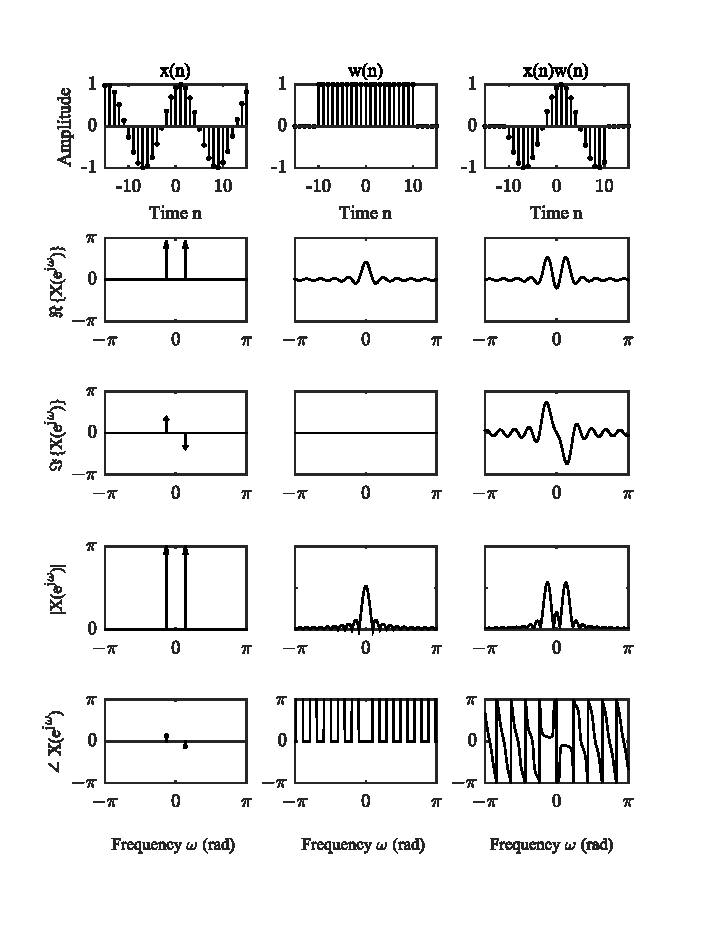
\includegraphics{figures/figure3_1.eps}
	\vspace{-0.6cm}
	\caption{Visualization of window impact on a sinusoid $x(n)=\cos(\omega_0 n+\phi)$ in time and frequency domain with $\omega_0=0.1\cdot2\pi$ and $\phi=-\pi/8$ and a rectangular window with length $N_w=21$. The window \gls{DTFT}T $W(e^{j\omega})$ is shifted dependent on $\omega_0$ and multiplied by $e^{j\phi}$ and $e^{-j\phi}$, respectively, as shown in the phase response of $\text{\gls{DTFT}T}\left(x(n)w(n)\right)$}\label{Figure31}
\end{figure}
%%%%%%%%%%%%%%%%%%%%%%%%%%%%%%%%%%%%%%

\noindent The left column of Figure~\ref{Figure31} represents the sequence $x(n)$ along time $n$ followed by its \gls{DTFT}T representation with real $\Re\{X(e^{j\omega})\}$ and imaginary $\Im\{X(e^{j\omega})\}$ parts as well as magnitude $|X(e^{j\omega})|$ and phase $\angle X(e^{j\omega})$ response. We set $\omega=0.1\cdot2\pi$ and $\phi=-\pi/8$.\\

\noindent The result in \eqref{eq:c3.4} is valid for an observation range of $n$ within $n\in]-\infty,\infty[$. In practice only a subset of samples $n$ is available for analysis. This limitation can be represented by introducing an \index{analysis!window}analysis window function which is multiplied with the sequence $x(n)$. The modest \index{window!rectangular, uniform, boxcar}analysis window is the rectangular, also known as boxcar or uniform window which has the value of one within the range of $N_w$ and zero outside
\begin{equation}\label{eq:c3.5}
w(n)=\begin{cases}1, & |n|\leq\frac{N_w-1}{2},\\
0, & \text{else},
\end{cases}
\end{equation}
for odd $N_w$.
This window is \index{symmetric}symmetric $(w(n)=w(-n))$ and has the \index{zero!-phase}\index{phase!zero-phase}zero-phase property, yielding a real-valued \gls{DTFT}T of the analysis window
\begin{equation}\label{eq:c3.6}
W(e^{j\omega})=\sum_{n=-\infty}^{\infty}w(n)e^{-j\omega n}=\sum_{n=-(N_w-1)/{2}}^{(N_w-1)/{2}}1e^{-j\omega n}=\frac{\sin\left(\frac{N_w\omega}{2}\right)}{\sin\left(\frac{\omega}{2}\right)},
\end{equation}
also known as \index{Dirichlet kernel}\textit{Dirichlet kernel}. The middle column of Figure~\ref{Figure31} illustrates a \index{symmetric}symmetric rectangular window in time and frequency domain with length $N_w=21$ and a \gls{DTFT}T length of $N=31$ (continuous line). The real part is equal to the Dirichlet kernel and the imaginary part is equal to zero due to the symmetry of the window $w(n)$. The phase response represents the sign of $W(e^{j\omega})$ dependent on $\omega$ and is equal to zero within the mainlobe width.\\
% Analyzing $x(n)$ within a limited range of $n\in[-\frac{N_w-1}{2},\frac{N_w-1}{2}]$ is equivalent of multiplying $x(n)$ with the analysis window $w(n)$.

\noindent The product $x(n)w(n)$ corresponds to a convolution in the frequency domain according to
\begin{equation}\label{eq:c1.7}
X_w(e^{j\omega})=\text{\gls{DTFT}T}\left(x(n)w(n)\right)=\left\{X\ast W\right\}(e^{j\omega}).
\end{equation}

\begin{mdframed}
	\begin{lstlisting}[language = Tex, caption={Add formulars to your text}]
	\begin{equation}\label{eq:c1.7}
	X_w(e^{j\omega})=\text{\gls{DTFT}T}\left(x(n)w(n)\right)=\left\{X\ast W\right\}(e^{j\omega}).
	\end{equation}
	\end{lstlisting}
	By adding a label to your equation, you will be able to refer to the equation within the text!
\end{mdframed}

\noindent Plugging $X(e^{j\omega})$ and $W(e^{j\omega})$, derived in \eqref{eq:c3.3} and \eqref{eq:c3.6}, respectively, in \eqref{eq:c1.7} yields the following expression
\begin{equation}\label{eq:c3.8}
X_w(e^{j\omega})=\pi e^{j\phi}W(e^{j(\omega-\omega_0)})+\pi e^{-j\phi}W(e^{j(\omega+\omega_0)}).
\end{equation}

%%%%%%%%%%%%%%%%%%%%%%%%%%%%%%%%%%%%%%
%%%%%%%%%%%%% FIGURE 3.2 %%%%%%%%%%%%%
\begin{figure}[ht]
	\center % 20 587 530 727
	\includegraphics{figures/figure3_2.eps}
	% \includegraphics{Ch3/Figures/figure3_2.eps}
	\vspace{-0.6cm}
	\caption{Relation of sinusoidal periods and window length and its impact on amplitude and phase: (a) shows a sinusoid multiplied by a boxcar window with a length of one period $(m=1)$. The Dirichlet kernels do not interfere at $\omega=\omega_0$ and $\omega=-\omega_0$ which yields an unbiased phase estimate of $\angle X_w(e^{j\omega_0})=\phi$, (b) presents the more general case of a window length which does not correspond to an integer multiplier of the sinusoids period $(m=1.1)$. The amplitude as well as the phase do not approach the true value and thus, the outcome is biased.}\label{Figure32}
\end{figure}
%%%%%%%%%%%%%%%%

\begin{mdframed}
	\begin{lstlisting}[language = Tex, language = Tex, caption={Example on how to add a figure to your text}]
	\begin{figure}
		\center % 20 587 530 727
		\includegraphics{figures/figure3_2.eps}
		\vspace{-0.6cm}
		\caption{Relation of sinusoidal periods and window length and its impact on amplitude and phase: (a) shows a sinusoid multiplied by a boxcar window with a length of one period $(m=1)$. ...}\label{Figure32}
	\end{figure}
	\end{lstlisting}
	By adding a label to your figure, you will be able to refer to the figure within the text!
\end{mdframed}

This is a rather important observation as the Dirichlet kernels are shifted along the frequency axis to $\omega=\omega_0$ and $\omega=-\omega_0$. The multiplication by the constants $e^{j\phi}$ and $e^{-j\phi}$, respectively, yields a complex valued $X_w(e^{j\omega})$ as shown in the right column of Figure~\ref{Figure31}. The terms on the right-hand-side of \eqref{eq:c3.8} constructively add or eliminate each other, dependent on the value of $\phi$ and $\omega_0$, described as \index{leakage effect}\emph{leakage effect}.\\

\noindent The interaction between the Dirichlet kernels is minimized if the frequency $\omega_0$ fulfills the following requirement
\begin{equation}\label{eq:c3.9}
\omega_0=\frac{2{m}\pi}{N_w}, \quad m\in\mathbb{N}.
\end{equation}
with $m$ denoting the number of periods contained in one window length $N_w$. Figure~\ref{Figure32} illustrates the impact of $\omega$ on the resulting magnitude and phase response of one sinusoid $x(n)=\cos(\omega_0 n+\phi)$ with $\phi=-\pi/8$, multiplied by a symmetric window of length $N_w=31$. Setting $\omega_0=1\frac{2\pi}{N_w}$ leads to $m=1$ and for the phase response at frequency $\omega=\omega_0$ we obtain
\begin{equation}
X_w(e^{j\omega_0})=\pi e^{j\phi}W(e^{j(\omega_0-\omega_0)})+\pi e^{-j\phi}W(e^{j(\omega_0+\omega_0)})\\
\end{equation}
As the \gls{DTFT}T of the rectangular window $W(e^{j2\omega_0})=0$ for $m\in\mathbb{N}$, the phase response yields the true value of $\phi$ at frequency $\omega_0$.
\begin{align}\label{eq:c3.10}
	X_w(e^{j\omega_0})&=\pi e^{j\phi} CG\\
	\angle X_w(e^{j\omega_0})&=\phi,
\end{align}
with defining $CG=W(e^{j0})$ as the \index{coherent gain}{coherent gain} for the selected window\footnote{Using a footnote you can associate you can give the reader the opportunity, to search for alternative sources}. The right column of Figure~\ref{Figure32} demonstrates the more general case of $m\notin\mathbb{N}$. The sidelobs of $W(e^{j\omega})$ interact with each other, resulting in a \index{bias}biased phase response at $\omega_0$. Note, that the peak's location of the magnitude response is not at $\omega_0$ due to the complex-valued superposition of both kernels. Therefore, any \index{peak-picking}peak-picking method for obtaining a sinusoidal phase would result in a biased outcome.\\

\noindent In order to reduce the unpleasant impact of the sidelobe level, the choice of the window type becomes of particular interest. Basically, their behavior can be categorized by two characteristics: \index{leakage effect}{spectral leakage} and {frequency resolution}. The frequency resolution is limited by the mainlobe width which corresponds to the ability to resolve two adjacent spectral lines. To increase the frequency resolution a window function with a small mainlobe width is preferred. As a smaller mainlobe width is on the expense of a reduced sidelobe level the choice of an appropriate window function is a trade-off between a high frequency resolution and a low sidelobe level. Another way of optimizing the window choice is to adjust the window length $N_w$ to fulfill the requirement in \eqref{eq:c3.9}. However, adapting $N_w$ needs knowledge of $\omega_0$ and is in general only possible for one single sinusoid. \\

\noindent Figure~\ref{Figure33} shows the influence of three prominent window types on the amplitude and phase response of the sequence $x_w(n)=\sin(\omega_0 n+\phi)w(n)$ with $\omega=3.1\cdot 2\pi/N_w$ and $\phi=-\pi/8$. So far, only the rectangular window was discussed. Its high frequency resolution ($6\,\text{dB}$ bandwidth of the mainlobe width: $\Delta\omega_{\text{MW}}=1.21\cdot 2\pi/N_w$) is at the cost of rather poor sidelobe suppression level of $-13\,\text{dB}$ for the strongest neighboring sidelobe (Fig.~\ref{Figure33} a)). The widely used Hamming window (b) consists of three shifted Dirichlet kernels with the purpose to minimize the sidelobe levels, achieving a suppression of $-42\,\text{dB}$ at the cost of a worse frequency resolution ($6\,\text{dB}$ bandwidth of mainlobe: $\Delta\omega_{\text{MW}}=1.81\cdot 2\pi/N_w$). The amplitude and phase response of the Hamming-windowed sinusoid reveal the advantage of a higher sidelobe suppression. The phase response at frequencies within the mainlobe width
is determined by the true phase value $\phi=-\pi/8$.
Compared to the rectangular window, the employment of a \index{window!Hamming}Hamming window results in a more robust phase estimation if an inaccurate frequency estimate of the sinusoid is given. Further, the magnitude's peak location is less shifted which yields a more accurate phase estimation when using \index{peak-picking}peak-picking. Finally, the \index{window!Blackman}{Blackman} window is presented in (c) with a sidelobe suppression of $-58\,\text{dB}$ and a $6\,\text{dB}$ mainlobe bandwidth of $\Delta\omega_{\text{MW}}=2.35\cdot 2\pi/N_w$. The neighboring phase values at $\omega_0$ are strongly influenced by the true phase value of $\phi$. However, both Hamming and Blackman windows deal with an increased mainlobe width. Once we extend our signal to multiple sinusoids, the mainlobe width plays a major role in selecting an appropriate window. If the mainlobe width contains more than one sinusoid then it is no longer possible to resolve the phase values of the sinusoids.

%%%%%%%%%%%%% FIGURE 3.3 %%%%%%%%%%%%%
\begin{figure}[t]
	\center % 20 587 530 727
	\includegraphics{figures/figure3_3.eps}
	% \includegraphics{Ch3/Figures/figure3_3.eps}
	% \vspace{-0.6cm}
	\caption{Illustration of different windows' impact on the magnitude and phase response of one sinusoid. The improved sidelobe suppression is at the cost of a higher mainlobe width resulting in a lower frequency resolution. For windows with higher sidelobe suppression, the phase response at frequency $\omega_0$ is increasingly dominated by the phase $\phi$ within the mainlobe width.}\label{Figure33}
\end{figure}
%%%%%%%%%%%%%%%%

\subsection{Example 2: discrete-time sinusoid in noise}~\\

%%%%%%%%%%%%% FIGURE 3.4 %%%%%%%%%%%%%
\begin{figure}[t]
	\center % 20 587 530 727
	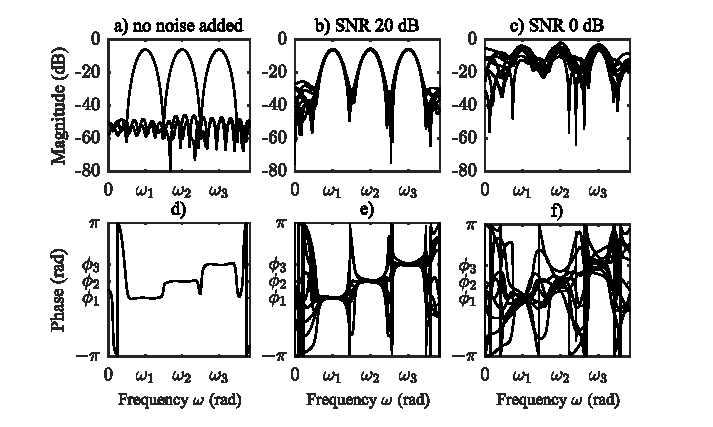
\includegraphics{figures/figure3_4.eps}
	\caption{Illustration of the impact of additive white Gaussian noise on the magnitude and phase response of three neighboring sinusoids, windowed with Hamming.}\label{Figure34}
\end{figure}
%%%%%%%%%%%%%%%%

So far, one sinusoid without additive noise was considered. For practical scenarios, the signal of interest is composed of multiple sinusoids corrupted with noise as shown in Figure~\ref{Figure34}. The problem to solve is the estimation of the sinusoidal phase ${\phi}_{h}$ given its amplitude and frequency denoted as $A_h$ and ${\omega}_h$, respectively. Following the harmonic model of a speech signal we assume that the sinusoidal frequency ${\omega}_h$ is constrained to be a multiple harmonic of a fundamental frequency, i.e. ${\omega}_h=h{\omega}_0$ with $h\in[1,\ldots,H]$ denoting the harmonic index
\begin{equation}\label{eq:c3.11}
x(n)=\sum_{h=1}^H{A_h\cos({\omega}_hn+{\phi}_h)}+d(n),
\end{equation}
with $\omega_h=h2\pi f_0/f_s$ and $d(n)$ as the additive noise. Application of a window function $w(n)$, having non zero values in the range of $[-(N_w-1)/2,(N_w-1)/2]$, yields the windowed signal $x_w(n)=x(n)w(n)$. Similar to \eqref{eq:c3.8}, the \gls{DTFT}T spectrum follows as
\begin{equation}\label{eq:c3.12}
X_w(e^{j\omega})=\sum_{h=1}^{H} A_h\pi \left( e^{j{\phi}_h}W(e^{j(\omega-{\omega}_h)}) + e^{-j{\phi}_h}W(e^{j(\omega+{\omega}_h)})\right)+D_w(e^{j\omega}),
\end{equation}
where $D_w(e^{j\omega})=\sum_{n=-(N_w-1)/2}^{(N_w-1)/2}{d(n)w(n)e^{-j{\omega}n}}$ and $W(e^{j\omega})$ is the window frequency response. To have a better insight into the phase estimation problem, we are interested in the effect of the neighboring harmonics $h\neq \bar{h}$ on the desired harmonic $\bar{h}$. We evaluate the frequency response of $X(e^{j\omega_{\bar{h}}})$ at the desired frequency ${\omega}_{\bar{h}}$
\begin{equation}\label{eq:c3.13}
\begin{split}
X_w(&e^{j\omega_{\bar{h}}})=A_{\bar{h}}\pi e^{j{\phi}_{\bar{h}}}\cdot CG+A_{\bar{h}}\pi e^{-j{\phi}_{\bar{h}}}W(e^{j2\omega_{\bar{h}}})\\
&+\sum_{h=1,h\neq{\bar{h}}}^H {A_h\pi e^{j{\phi}_h}W(e^{j(\omega_{\bar{h}}-\omega_h)})+A_h\pi e^{-j{\phi}_h}W(e^{j(\omega_{\bar{h}}+\omega_h)}})+D_w(e^{j\omega_{\bar{h}}}).
\end{split}
\end{equation}
The additive terms on the right-hand-side of Equation \eqref{eq:c3.13} show the interaction of the adjacent harmonics to the desired phase $\phi_{\bar{h}}$ as well as the impact of the additive noise. In the following we are interested in the influence of these terms on the desired phase by re-writing \eqref{eq:c3.13} according to
%%%%%%%%%%%%%%%%
%TODO \input{Chapters/Captions/Figures/figure3_5}

\begin{equation}\label{eq:c3.14}
X_w(e^{j\omega_{\bar{h}}})=X_r(e^{j\omega_{\bar{h}}})e_c
\end{equation}
where $X_r(e^{j\omega_{\bar{h}}})=A_{\bar{h}}\pi e^{j\phi_{\bar{h}}}$ and $e_c$ captures the phase estimation errors, given by
\begin{eqnarray}\label{eq:c3.15}
e_c&=&\sum_{h=1}^H\frac{A_h}{A_{\bar{h}}}\left( e^{j(\phi_h-\phi_{\bar{h}})}W(e^{j(\omega_{\bar{h}}-\omega_h)})+ e^{-j(\phi_h+\phi_{\bar{h}})}W(e^{j(\omega_{\bar{h}}+\omega_h)}) \right)\nonumber\\
&+& \frac{1}{\pi A_{\bar{h}}}e^{-j\phi_{\bar{h}}}D_w(e^{j\omega_{\bar{h}}})
\end{eqnarray}
In order to get more insight on the phase error term $e_c$, in the following we derive its phase mean and variance.\\
\textbf{First moment of }$\boldsymbol{e_c}$~\\
\noindent The mean value of the phase error term is given by
\begin{equation}\label{eq:c3.16}
\mathbb{E}_\phi(e_c)=\int_{-\pi}^\pi e_c p(\phi)d\phi
\end{equation}
with $p(\phi)$ denoting the phase distribution. Applying \eqref{eq:c3.16} to \eqref{eq:c3.15} the first moment of $e_c$ is given by
\begin{equation}\label{eq:c3.17}
\begin{split}
\mathbb{E}_\phi(e_c) &= \sum_{h=1}^H\frac{A_h}{A_{\bar{h}}} \mathbb{E}(e^{j(\phi_h-\phi_{\bar{h}})})W(e^{j(\omega_{\bar{h}}-\omega_h)})\\
&+ \sum_{h=1}^H\frac{A_h}{A_{\bar{h}}} \mathbb{E}(e^{-j(\phi_h+\phi_{\bar{h}})})W(e^{j(\omega_{\bar{h}}+\omega_h)})\\
&+ \frac{1}{\pi A_{\bar{h}}}\mathbb{E}(e^{-j\phi_{\bar{h}}})D_w(e^{j\omega_{\bar{h}}})
\end{split}
\end{equation}
\textbf{Second moment of }$\boldsymbol{e_c}$~\\
\noindent \index{phase!error variance}The second moment of the error term is given by
\begin{equation}\label{phasevar0}
\begin{split}
\mathbb{E}_\phi\left(e_c e_c^*\right)&=\!\sum_{h_1=1}^{H-1} \sum_{h_2=h_1+1}^H \! C_1(\bar{h},h_1,h_2) \mathbb{E}_\phi\!\left(\cos(\phi_{h_1} \!-\! \phi_{h_2} \!+\!\angle w_1(\bar{h},h_1,h_2))\right)\\
&+ \!\sum_{h_1=1}^{H-1} \sum_{h_2=h_1+1}^H\!C_2(\bar{h},h_1,h_2)\mathbb{E}_\phi\!\left(\cos(\phi_{h_1} \!-\! \phi_{h_2} \!-\!\angle w_2(\bar{h},h_1,h_2))\right)\\
&+ \!\sum_{h_1=1}^H \sum_{h_2=1}^H\!C_3(\bar{h},h_1,h_2)\mathbb{E}_\phi\!\left(\cos(\phi_{h_1} \!+\! \phi_{h_2} \!+\!\angle w_3(\bar{h},h_1,h_2))\right)\\
&+\sum_{h=1}^H C_4(\bar{h},h)\mathbb{E}_\phi\left(\cos(\phi_h-\phi_{\bar{h}}+\angle W(e^{j(\omega_{\bar{h}}-\omega_h)})D_w(e^{-j\omega_{\bar{h}}}))\right)\\
&+\sum_{h=1}^H C_5(\bar{h},h)\mathbb{E}_\phi\left(\cos(\phi_h+\phi_{\bar{h}}-\angle W(e^{j(\omega_{\bar{h}}+\omega_h)})D_w(e^{-j\omega_{\bar{h}}}))\right)\\
&+\frac{1}{\pi^2A_{\bar{h}}^2}|D_w(e^{j\omega_{\bar{h}}})|^2 + C_6(\bar{h}),
\end{split}
\end{equation}
\begin{mdframed}
	\begin{lstlisting}[language = Tex, caption={Add formulars to your text, splitted equations}]
	\begin{equation}\label{phasevar0}
	\begin{split}
	\mathbb{E}_\phi\left(e_c e_c^*\right)&=\!\sum_{h_1=1}^{H-1} \sum_{h_2=h_1+1}^H \! C_1(\bar{h},h_1,h_2) \mathbb{E}_\phi\!\left(\cos(\phi_{h_1} \!-\! \phi_{h_2} \!+\!\angle w_1(\bar{h},h_1,h_2))\right)\\
	&+ \!\sum_{h_1=1}^{H-1} \sum_{h_2=h_1+1}^H\!C_2(\bar{h},h_1,h_2)\mathbb{E}_\phi\!\left(\cos(\phi_{h_1} \!-\! \phi_{h_2} \!-\!\angle w_2(\bar{h},h_1,h_2))\right)\\
	&+ \!\sum_{h_1=1}^H \sum_{h_2=1}^H\!C_3(\bar{h},h_1,h_2)\mathbb{E}_\phi\!\left(\cos(\phi_{h_1} \!+\! \phi_{h_2} \!+\!\angle w_3(\bar{h},h_1,h_2))\right)\\
	&+\sum_{h=1}^H C_4(\bar{h},h)\mathbb{E}_\phi\left(\cos(\phi_h-\phi_{\bar{h}}+\angle W(e^{j(\omega_{\bar{h}}-\omega_h)})D_w(e^{-j\omega_{\bar{h}}}))\right)\\
	&+\sum_{h=1}^H C_5(\bar{h},h)\mathbb{E}_\phi\left(\cos(\phi_h+\phi_{\bar{h}}-\angle W(e^{j(\omega_{\bar{h}}+\omega_h)})D_w(e^{-j\omega_{\bar{h}}}))\right)\\
	&+\frac{1}{\pi^2A_{\bar{h}}^2}|D_w(e^{j\omega_{\bar{h}}})|^2 + C_6(\bar{h}),
	\end{split}
	\end{equation}
	with the abbreviations
	\begin{equation}
	\begin{split}
	w_1(\bar{h},h_1,h_2)&=W(e^{j(\omega_{\bar{h}}-\omega_{h_1})})W(e^{-j(\omega_{\bar{h}}-\omega_{h_2})}),\\
	w_2(\bar{h},h_1,h_2)&=W(e^{j(\omega_{\bar{h}}+\omega_{h_1})})W(e^{-j(\omega_{\bar{h}}+\omega_{h_2})}),\\
	w_3(\bar{h},h_1,h_2)&=W(e^{j(\omega_{\bar{h}}-\omega_{h_1})})W(e^{-j(\omega_{\bar{h}}+\omega_{h_2})}),
	\end{split}
	\end{equation}
	\end{lstlisting}
	By adding a label to your equation, you will be able to refer to the equation within the text!
\end{mdframed}
with the abbreviations
\begin{equation}
\begin{split}
w_1(\bar{h},h_1,h_2)&=W(e^{j(\omega_{\bar{h}}-\omega_{h_1})})W(e^{-j(\omega_{\bar{h}}-\omega_{h_2})}),\\
w_2(\bar{h},h_1,h_2)&=W(e^{j(\omega_{\bar{h}}+\omega_{h_1})})W(e^{-j(\omega_{\bar{h}}+\omega_{h_2})}),\\
w_3(\bar{h},h_1,h_2)&=W(e^{j(\omega_{\bar{h}}-\omega_{h_1})})W(e^{-j(\omega_{\bar{h}}+\omega_{h_2})}),
\end{split}
\end{equation}
and the phase independent constants 
\begin{equation}
\begin{split}
C_1(\bar{h},h_1,h_2)&=2\frac{A_{h_1} A_{h_2}}{A^2_{\bar{h}}}|w_1(\bar{h},h_1,h_2)|,\\
C_2(\bar{h},h_1,h_2)&=2\frac{A_{h_1} A_{h_2}}{A^2_{\bar{h}}}|w_2(\bar{h},h_1,h_2)|,\\
C_3(\bar{h},h_1,h_2)&=2\frac{A_{h_1} A_{h_2}}{A^2_{\bar{h}}}|w_3(\bar{h},h_1,h_2)|,\\
C_4(\bar{h},h)&=2\frac{A_h}{\pi A^2_{\bar{h}}}|W(e^{j(\omega_{\bar{h}}-\omega_h)})||D_w(e^{j\omega_{\bar{h}}})|,\\
C_5(\bar{h},h)&=2\frac{A_h}{\pi A^2_{\bar{h}}}|W(e^{j(\omega_{\bar{h}}+\omega_h)})||D_w(e^{j\omega_{\bar{h}}})|,\\
C_6(\bar{h})&=\sum_{h=1}^H \frac{A_h^2}{A_{\bar{h}}^2}\left( |W(e^{j(\omega_{\bar{h}}+\omega_{{h}})})|^2+|W(e^{j(\omega_{\bar{h}}-\omega_{{h}})})|^2 \right).
\end{split}
\end{equation}
The second moment of the phase error in \eqref{phasevar0} provides useful insights on how the phase of the desired frequency $\omega_{\bar{h}}$ is a function of the chosen window, the additive noise and the neighboring harmonics. Subsequently the key factors are summarized as
\begin{itemize}
	\item $W(e^{j\omega})$ the magnitude and phase response of the \index{analysis!window}analysis window function
	\item $D_w(e^{j\omega})$ the magnitude and phase response of the additive noise
	\item $\frac{A_h}{A_{\bar{h}}}$ the amplitude ratio of the adjacent and desired harmonics
\end{itemize}
The impact of the selected window $W(e^{j\omega})$ can be considered for two cases: First, the harmonics are separated sufficiently which means there is no neighboring harmonic within the mainlobe width. The window's amplitude $W(e^{j(\omega_{\bar{h}}-\omega_h}))$ for $\bar{h}\neq h$ suppresses the neighboring harmonic by its sidelobe level (see Figure~\ref{Figure33}) which results in a low impact of the neighboring harmonics to $\hat{\phi}$. If the harmonics are not separated, i.e., the adjacent harmonic is located within the mainlobe width then the phase error gets larger. The adjacent harmonic is not attenuated by the sidelobe level of the window thus the phase estimation gets more 